\documentclass[pdflatex,ja=standard]{bxjsarticle}

% Language setting
% Replace `english' with e.g. `spanish' to change the document language
\usepackage[japanese]{babel}
\usepackage{graphicx} % Required for inserting images
\usepackage{amsmath}
\usepackage{amssymb}
\usepackage{xeCJK}
\usepackage{listings}
\usepackage{autobreak}
\begin{document}
1.1 (a)

\begin{equation}
p(y) = \frac{1}{2} \cdot \frac{1}{\sqrt{2 \pi \cdot 2^2}} \exp{ \{ \frac{(y-1)^2}{2 \cdot 2^2} \}} + \frac{1}{2} \cdot \frac{1}{\sqrt{2 \pi \cdot 2^2}} \exp{ \{ \frac{(y-2)^2}{2 \cdot 2^2} \} }
\end{equation}

\begin{lstlisting}
#%%
import numpy as np
import matplotlib.pyplot as plt

def norm_dist(x: np.ndarray, mu: float, sigma: float) -> np.ndarray:
    return 1 / (sigma * np.sqrt(2 * np.pi)) * np.exp(- 1./2 * ((x - mu) / sigma) **2)

#%% 
x = np.linspace(-10, 10, 1000)
y1 = norm_dist(x, 1, 2)
y2 = norm_dist(x, 2, 2)

y = 1/2 * y1 + 1/2 * y2
plt.plot(x, y)
plt.show()

\end{lstlisting}

\begin{figure}
    \centering
    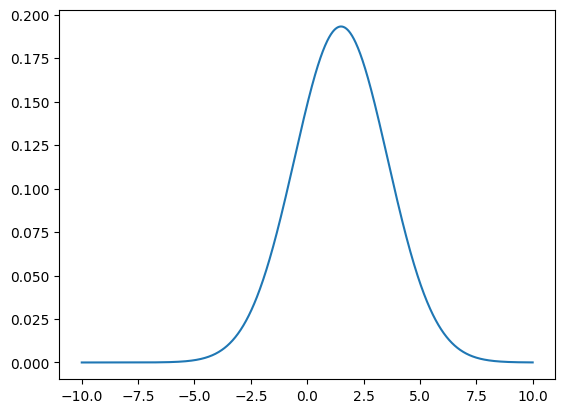
\includegraphics[width=0.5\linewidth]{norm_dist.png}
    \caption{1.1.(a) の描画結果}
    \label{fig:placeholder}
\end{figure}

1.1(b)
\begin{gather}
\rm{Pr} (\theta = 1 | y = 1) = \frac{Pr(\theta = 1) Pr(y=1 |\theta = 1) }{Pr(y=1)} \\
=  \frac{\exp(-\frac{(1-1)^2}{2 \cdot 2^2} ) }{\exp(-\frac{(1-1)^2}{2 \cdot 2^2}) + \exp(-\frac{(1-2)^2}{2 \cdot 2^2})} \\
= \frac{1}{1 + \exp(-0.125)} = 0.531
\end{gather}

1.1(c) \\
1.1(b)同様の式展開により、
\begin{gather}
\rm{Pr} (\theta = 1 | y) = \frac{\exp(-\frac{(y-1)^2}{2 \sigma^2} ) }{\exp(-\frac{(y-1)^2}{2 \sigma ^2}) + \exp(-\frac{(y-2)^2}{2 \sigma^2})} \\
= \frac{1}{1 + \exp(-\frac{-2y + 3}{2 \sigma^2})}
\end{gather}
$ f(x) = 1 / (1 +\exp(-\frac{x}{\sigma}))$ のグラフのスケールを変えて描画してみると、$\theta$の事後分布は$\sigma$が小さくなるほど0か1の両極端な分布となり、大きくなるほど $\rm{Pr} (\theta = 1|y) = \rm{Pr} (\theta = 2|y) = 0.5$ と偏りのない分布に近づくことがわかる。

\begin{lstlisting}
#%%
import numpy as np
import matplotlib.pyplot as plt

def func(x: np.ndarray, sigma: float) -> np.ndarray:
    return 1 / (1 + np.exp(-x / sigma))

#%% 
x = np.linspace(-10, 10, 1000)
y1 = func(x, 0.01)
y2 = func(x, 0.1)
y3 = func(x, 10)
y4 = func(x, 100)

plt.plot(x, y1, label="sigma=0.01")
plt.plot(x, y2, label="sigma=0.1")
plt.plot(x, y3, label="sigma=10")
plt.plot(x, y4, label="sigma=100")
plt.legend()
plt.show()
\end{lstlisting}

\begin{figure}
    \centering
    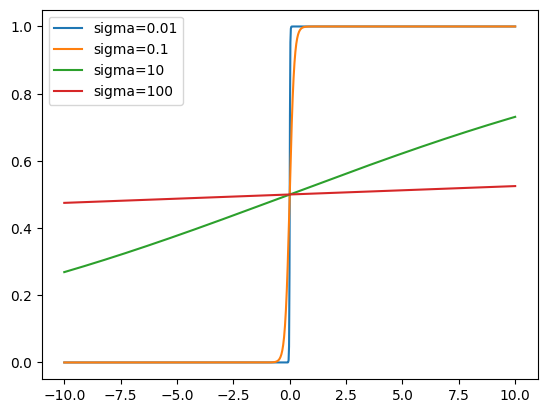
\includegraphics[width=0.5\linewidth]{output_sigmoid_like.png}
    \caption{1.1(c)の描画結果}
    \label{fig:placeholder}
\end{figure}

1.6

\begin{gather}
\rm{Pr} (\mbox{一卵性双生児} | \mbox{男同士の双子である}) = \frac{Pr(\mbox{一卵性双生児かつ男同士である})}{\rm{Pr}(\mbox{男同士の双子である})} =\\
\frac{\rm{Pr}(\mbox{一卵性双生児かつ男同士である})}{\rm{Pr}(\mbox{一卵性双生児の男同士})+Pr(\mbox{二卵性双生児の男同士})} \\
= \frac{\rm{Pr}(\mbox{一卵性双生児})\cdot1/2}{\rm{Pr}(\mbox{一卵性双生児})\cdot1/2 + Pr(\mbox{二卵性双生児})\cdot 1/4} = \frac{1/300}{1/300+1/125 \cdot 1/2} = 0.455
\end{gather}
よって45.5\%。

1.7

箱を変える場合は 

$\rm{Pr}(\mbox{豪華な商品を得る}|\mbox{箱を変える}) = \frac{Pr(\mbox{箱を変える、かつ豪華な商品を得る})}{Pr(\mbox{箱を変える})} = 2/3. $

$ \because $ 豪華な商品の箱への入り方3通りと最初の箱を選ぶ3通りを併せて合計9通りの組み合わせを考えると、豪華な商品を選ぶ確率は、最初に豪華な商品の箱を\textgt{選ばなかった}ときのみ $ =(9-3)/9 = 6/9 = 2/3. $

箱を変えない場合は反対に、最初に豪華な商品の箱を\textgt{選んだ}ときのみ得られるため、 

$\rm{Pr}(\mbox{豪華な商品を得る}|\mbox{箱を変えない}) = \frac{\rm{Pr}(\mbox{箱を変えない、かつ豪華な商品を得る})}{Pr(\mbox{箱を変えない})} = 3/9 = 1/3.$

1.8

(a) Aが観察したサイコロの目の手順にたまたま6が多かったら、$P(E|I_A) > 1/6$ とするのが妥当だろう。
しかし、Bは知識を持っていないので、$P(E|I_B) = 1/6$ と推定するだろう。

(b) Aは無知なので、ワールドカップの出場国数を$N$とすると $P(E|I_A) = 1/N$ と推定するが、
一方でBはブラジルが過去に優れた戦績を挙げているという情報をもとに、$P(E|I_B)$を$1/N$ よりもはるかに大きい値に設定することが予想される。

1.9

(a)コード "1-9.py" を実行した結果、44人の患者が来院し、42人が待たないといけなかった。平均待ち時間は76.4分で、診療所は午前9時から586分後つまり午後6時46分に閉院した。

(b)コード "1-9.py" を実行した結果は下記の通り。

\begin{lstlisting}
43.0 40.0 66.43857093736227 554.565324530271
       num_patients  num_wait_patients  mean_waiting_times  \
count    100.000000         100.000000          100.000000   
mean      43.300000          40.570000           72.635895   
std        7.165433           8.498669           39.271592   
min       26.000000          17.000000            7.486453   
25%       39.000000          36.000000           43.478445   
50%       43.000000          40.000000           66.438571   
75%       47.250000          46.000000           93.654827   
max       66.000000          65.000000          207.551080   

       total_consult_times  
count           100.000000  
mean            568.319741  
std              78.700268  
min             440.750080  
25%             515.398373  
50%             554.565325  
75%             614.927855  
max             860.047157  
\end{lstlisting}

\end{document}
